\chapter{Characterization of the Mechanical Properties of Soft Materials} \label{ch:characterizationSoft}

% \textbf{ \huge To-Do List}

% Explain characterization process following a systematic approach:
% \begin{itemize}
%     \item Describe the stress relaxation test. Mention the parameters collected. Compile in a table the deformation to which each material was held during the test. Mention that initially the test duration was longer than the one being used for fitting the mathematical model.
%     \item Describe now the pre-processing done to the collected raw data. Several conditions were established to decide how much to smooth the raw data.
%     \item Present the obtained stress relaxation curves
% \end{itemize}

% Things to explain
% \begin{itemize}
%     \item Allowable attenuation of max value is 5 percent
%     \item (Done) Consider cell resolution for limiting the amount of attenuation in the smoothing algorithm to the right amount. (The load cell used provides accurate measurements up to 1/500 of its capacity, i.e. for a load cell of 50 kN the smallest accurate measurement is 100N. All the soft materials implemented have load values in the range of 1 to 100 N. Therefore, using the accuracy parameters of the load cell as a guide is not possible.)
% \end{itemize}

\section{Introduction}

Previously, the trend in soft robotic application for human assistance to mimic the human skeletal muscle system, which is mainly focus on the contractile element (CE) of the muscle-tendon component, was identified. Recently, research has been done on implementing soft materials as the elastic element of series-elastic actuators (SEAs). This is motivated by the fact that viscoelasticity, found in biological tissue and many soft materials, may be able to overcome current limitations on SEAs. This is inline with the literature, which states that polymers, such as polyethylene, have similar mechanical properties as the human tendon. The literature available on the concept of series-viscoelastic actuators (SVAs) is very scarce and is currently facing the challenge of accurately estimating the force/torque transmitted by soft materials, such as rubber. One of the aims of this research is to develop a modelling tool able to address the latter. Therefore, this chapter covers the following points.

Firstly, a selection of different off-the-shelf soft materials is made from the family of composite materials, specifically thermoplastic elastomers (TPEs). The selection is based on the literature, which suggest that this type of materials have similar viscoelastic properties as the human tendon. The materials are as follows: Polyethylene Rubber (PR), Ethylene Polypropylene Rubber (EPR), Natural Rubber with Polyester (NatPolR), Natural Rubber (NatR), Silicone Rubber (SR), Fluorocarbon Rubber (FR), and Nitrile Rubber (NR). All the materials were acquired from RS Components UK\textregistered{}, with the exception of the Natural Rubber, which was acquired from CoreZone Sports\textregistered{} in the form of resistance bands of different thickness.

Secondly, the mechanical property of viscoelasticity of this type of materials is discussed. Thirdly, the characterization of the mechanical properties of these materials is presented. In here, the mechanical tests of tensile strength and stress relaxation are performed to extract both the elastic and viscoelastic properties of the materials. As previously mentioned, the study of the creep and hysteresis effect is out of the scope of this research. Finally, the collected data was processed in Matlab\textregistered{} prior to creating the visual representation of the studied properties. 

\section{Mechanical Properties of Soft Materials} \label{sec:mechprop}

The soft materials studied in this work belong to the family of thermoplastic elastomers. Elastomers are created by mixing a thermoplastic material, such as natural or synthetic rubber, with other materials, such as carbon and sulfur. This process is called vulcanization which creates cross-linked structures inside the material. Since elastomers are based on rubber, the terms elastomer and rubber are often used interchangeably. Elastomers are known to have nonlinear stress response, low stiffness and to achieve high deformation lengths. Some elastomers can fully recover their shape after stretched many times their length. They are also known to exhibit both elastic and viscoelastic properties. The latter means the stress response of elastomers is also time-dependent \cite{Bauman2008}. The main mechanical properties of elastomers are described in following paragraphs.

\subsection{Elasticity}

Elasticity, or elastic behaviour, refers to the ability of a material to be deformed up to a certain length and completely recover its shape and dimensions when the load deforming it is removed. Elasticity also refers to ability of a material to comply with the law of constant proportionality between the stress and the strain, described by Hooke's Law. However, elastomers are not purely elastic materials and tend to have a nonlinear stress-strain response, i.e. they do not obey Hooke's Law over the whole range of strains in the sense that the proportionality between the stress and the strain does not remain constant. This typical nonlinear behaviour in the stress-strain curve of elastomers is illustrated in \Cref{fig:tensile}.

\begin{figure}[hbt!]
    \centering
    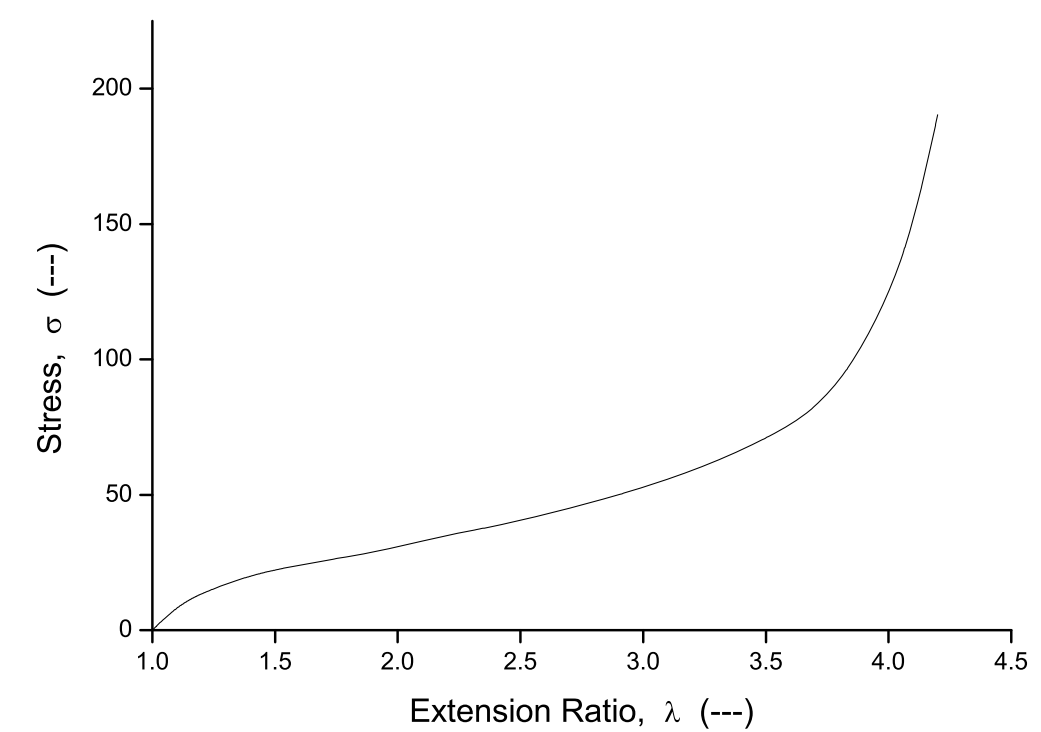
\includegraphics[width=0.7\textwidth]{TensileExample.png}
    \caption{Typical stress-strain curve of elastomers. \cite{Bauman2008}.}
    \label{fig:tensile}
\end{figure}

Elastomers exhibit elastic behaviour over a certain range of deformations, known as the elastic limit or elastic region. Beyond this limit the material is likely to undergo plastic or permanent deformation, this means the material will not recover its original shape completely. In some cases, the elastic limit is not easily visible on the stress-strain curve of a material, and instead the proportional limit is used to approximate the location of the elastic limit. The proportional limit is defined as the point in the stress-strain curve where the nonlinear response (change in the curve's slope) is first observed. Another way to approximate the elastic limit of a materials is using the yield strength, which is defined as the largest stress value on the curve, or the first point in which an increase in strain occurs without an increase in the stress \cite{ebewele2000}. These are some of the parameters that can be extracted from the tensile strength test and are useful to delimit the operating conditions of the materials. For this reason, particular care is put into accurately defining the elastic region, hence the safe operating conditions, of the studied soft materials. This is better described in SECTION. Also, this will facilitate the comparison analysis performed latter in this chapter.

\subsection{Viscoelasticity}

Viscoelasticity, is a property of some materials which are not purely elastic, do not fully obey Hooke's Law, nor purely viscous, do not fully obey Newton's Law, i.e. the stress is not proportional to the rate of change of the strain with time. In other words, the stress experienced by viscoelastic materials are dependent on both the amount and the speed of the strain applied to them. An example of a purely elastic material is a spring; whereas an example of a purely viscous material is a dashpot. The mechanical model of a viscoelastic material contains both elements, which can be arrange in different configurations. The set of mathematical models created out of these different configurations are known as the Linear Viscoelastic Models (LVMs). The time dependency or viscosity, of viscoelastic materials is appreciated in phenomenons such as creep, stress relaxation, hysteresis, the Mullin's Effect and in the Van der Waals forces.

Stress relaxation and creep are both time-dependent phenomenons observed in elastomers. On one hand, stress relaxation refers to the decrease over time of the stress experimented by a material when subjected to a constant strain (or deformation). On the other hand, creep refers to the increase over time of the material strain when subjected to a constant stress (or load). Understanding these phenomenons means understanding that elastomers are composed of a network of molecular chains. Inside this network, entanglements form naturally. According to J. Bauman in \cite{Bauman2008}, stress relaxation is mainly caused by the slipping of these entanglements ultimately causing a loosening of force applied by the network of molecular chains. Stress relaxation and creep occur in both constant and cyclic deformations. There are two mechanical tests designed to study these behaviours, from where it can be extracted the relaxation modulus and creep modulus of a material \cite{oberg2016}. 

Hysteresis in a material is defined as the mechanical energy dissipated as heat when the material is undergoing deformations. This phenomenon is observed in a loading-unloading cycle, where the stress trajectory of the material while loading (extension) is different than the trajectory during unloading (retraction), as illustrated in \Cref{fig:hysteresis}. Hysteresis is mainly caused by internal friction of the molecular chain, also known as Van der Waals forces, in both elongation and contraction. Van der Waals forces are caused by the momentary bonding experienced between molecular chains that are close together. This constant making and breaking of bonds caused by deforming a material produces heat which ultimately becomes a mechanism to dissipate mechanical energy. This energy is represented as the enclosed area in \Cref{fig:hysteresis}. Stress relaxation and creep play a role in the amount of hysteresis experienced by a material in each consecutive loading-unloading cycle. The effect of hysteresis alone can be isolated by subjecting the elastomer to a conditioning process (preconditioning) in which it undergo several loading-unloading cycles until the stress response stops changing with every new cycle.

\begin{figure}[htb!]
    \centering
    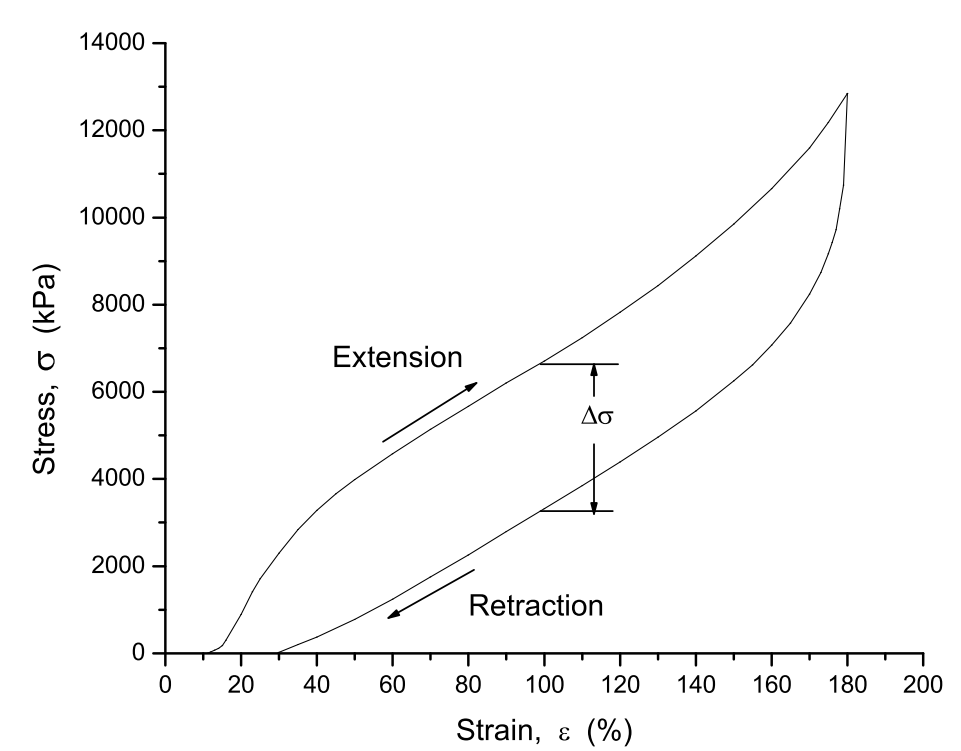
\includegraphics[width=0.8\textwidth]{HysteresisExample.png}
    \caption{Hysteresis in stress-strain curve. \cite{Bauman2008}.}
    \label{fig:hysteresis}
\end{figure}

The Mullin's effect is another important phenomenon in the mechanical behaviour of elastomers. This effect refer to the breakage of tense molecular chains resulted from the manufacturing process of the material. Therefore, the very first time the material is subjected to deformations it exhibits a larger stress response in comparison to consecutive deformations. The latter is also referred to as a weakening of the material. This effect is more dramatic than the stress relaxation but can be easily avoided when preconditioning the material. Having defined the expected mechanical properties of elastomers, the mechanical tests of tensile strength and stress relaxation are described in the following section.

\section{Characterization Process}

In this section, the mechanical tests of tensile strength and stress relaxation, performed as part of the characterization process, are described. The tests are performed in an Instron 3369 Dual Column Testing System equipped with a 50 kN load cell, at room temperature (25 \degree{} C). The experimental data is expected to contain some noise due to the accuracy limitations of the available load cell. The algorithm implemented to filter this noise is described in SECTION . As previously mentioned, the elastomers selected for this research are: Polyethylene Rubber, Ethylene Polypropylene, Natural Rubber with Polyester, Natural Rubber, Silicone Rubber, Fluorocarbon Rubber, and Nitrile Rubber. All the materials come in rectangular sheet form. Laser cutting was used to extract individual specimens from each material sheet with the layout illustrated in \Cref{fig:specimenLayout}, as recommended in the Standard Test Method for Vulcanized Rubbers - Tension (ASTM D412) \cite{astmd412}. Finally, all the specimens were preconditioned prior to testing by applying a small deformation to them.

\begin{figure}[htb!]
    \centering
    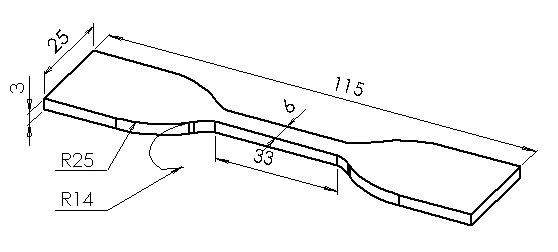
\includegraphics[width=0.6\textwidth]{SpecimenLayout.png}
    \caption{Specimen Type C Dumbbell Layout from the ASTM D412 \cite{astmd412}}
    \label{fig:specimenLayout}
\end{figure}

\subsection{Tensile Strength Test}

In a tensile strength test the material is loaded to failure at a certain deformation (strain) rate. The main purpose of this test is to extract the stress-strain curve of the material. From the stress-strain curve, the elastic properties of the material, such as stiffness, elastic modulus, ultimate strain, ultimate stress, elastic limit and yield strength, can be extracted. The stress-strain curve of elastomers, illustrated in  \Cref{fig:tensile}), has three main regions: the toe region, the elastic region, and the yield/failure region. In the toe region, the internal molecular chains of the material are misaligned, experiencing greater friction forces which greatly oppose to initial deformations. In contrast, when the molecular chains are aligned the friction forces decrease and the material deforms as a whole. The latter represent the elastic region, in which the slope of the curve (stiffness) is slightly smaller than in the toe-region. The elastic region of many materials exhibit a proportional or linear relationship between the stress and the strain. This is not the case for elastomers, where most of them exhibit a nonlinear relationship. When the internal molecular chains have been elongated to its maximum length they demand higher forces to fail, this is observed as a peak in the load-elongation curve which also highlights the beginning of the yield/failure region \cite{Bauman2008}.

The tensile strength test performed in this work is in accordance with the Standard Test Method for Vulcanized Rubbers - Tension (ASTM D412) \cite{astmd412}. Also, the Standard Test Method for Tensile Properties of Plastics (ASTM D638), was consulted on how to interpret the obtained stress-strain curves \cite{astmd638}. In here, it is recommended to elongate the material specimen until failure using a deformation rate of 500 mm/min, whenever possible. However, under certain circumstances where the previous deformation rate is not suitable, the test can be performed using the deformation rate of 250 mm/min. The latter was required for the silicon rubber, natural rubber and some resistance bands, where the gripper was not able to hold the material during the entirety of the test. In addition to the previous two deformation rates, a third one of 50 mm/min is used whenever possible. In summary, most of the materials are tested using at least two out of the three deformation rates of 50, 250 and 500 mm/min. The decision of characterizing the mechanical behaviour of the materials under different strain rates is motivated by the known velocity-dependency of the stress-response of this type of materials. This will be useful during the modelling stage. The exact number of tests performed to each material is summarized in \Cref{tbl:tensile_tests}.

\begin{table}[htb!]
    \centering
    \caption{Number of specimens used per type of test. All the resistance bands are made of 100 \% Natural Rubber and are color coding depending on their stiffness.}
    \begin{tabular}{lcccc}
    \toprule
    Type of Rubber & Thickness &  50 & 250 & 500\\
     & mm & mm/min & mm/min & mm/min \\
    \hline
    Ethylene Polypropylene   &  1.5 & 16 & - & 5\\
    Fluorocarbon              &  1.5 & 9 & 8 & 5\\
    Natural with Polyester   &  1.5 & 10 & 5 & -\\
    Nitrile                   &  1.5 & 7 & 7 & 5\\
    Silicone                  &  1.5 & 13 & 7 & 3\\
    Polyethylene              &  6 & 12 & 7 & 5\\
    \hline
    Natural - Yellow  & 0.33, 0.42 & 1 & 6 & 1\\
    Natural - Red  & 0.48, 0.52 & - & 8 & -\\
    Natural - Blue  & 0.64, 0.75 & - & 8 & -\\
    Natural - Green  & 0.97, 1.03 & - & - & 8\\
    Natural - Black  & 1.17, 1.31 & - & 6 & 2\\
    Natural - Orange  & 1.32, 1.49 & - & 5 & -\\
    \bottomrule
    \end{tabular}
    \label{tbl:tensile_tests}
\end{table}

% \begin{table}[htb!]
%     \centering
%     \caption{Tensile strength tests performed. All the resistance bands are made of 100 \% Natural Rubber and are color coding depending on their stiffness.}
%     % \begin{tabular}{|C{0.3\textwidth}||C{0.2\textwidth}|C{0.1\textwidth}|C{0.1\textwidth}|C{0.1\textwidth}|}
%     \begin{tabular}{lcccc}
%     \hline 
%     \multicolumn{5}{|c|}{Tensile Strength Datasets}\\
%     \hline
%     Type of Rubber & Thickness (mm) &   \multicolumn{3}{|c|}{ Deformation (mm/min)}\\
%     \cline{3-5}
%           &  & 50 & 250 & 500\\
%     \hline
%     Ethylene Polypropylene   &  1.5 & 16 & - & 5\\
%     Fluorocarbon              &  1.5 & 9 & 8 & 5\\
%     Natural with Polyester   &  1.5 & 10 & 5 & -\\
%     Nitrile                   &  1.5 & 7 & 7 & 5\\
%     Silicone                  &  1.5 & 13 & 7 & 3\\
%     Polyethylene              &  6 & 12 & 7 & 5\\
%     \hline
%     Natural - Yellow  & 0.33, 0.42 & 1 & 6 & 1\\
%     Natural - Red  & 0.48, 0.52 & - & 8 & -\\
%     Natural - Blue  & 0.64, 0.75 & - & 8 & -\\
%     Natural - Green  & 0.97, 1.03 & - & - & 8\\
%     Natural - Black  & 1.17, 1.31 & - & 6 & 2\\
%     Natural - Orange  & 1.32, 1.49 & - & 5 & -\\
%     \hline
%     \end{tabular}
%     \label{tbl:tensile_tests}
% \end{table}

The testing machine used for these experiments output the following parameters: reaction force, elongation, and time. In this work, the conventional parameters of stress, $\sigma$, and strain, $\varepsilon$, are used instead of the reaction force, $F$, and elongation, $\Delta L$. The latter is calculated using the initial length $l_o=33 mm$, and cross-sectional area (thickness times width), $A_o$, of the specimen, given in \autoref{fig:specimenLayout} and \autoref{tbl:tensile_tests}, respectively. Then it follows that $\sigma=F/A_o$, and $\varepsilon=l_o/\Delta L$.

\subsubsection{Data Processing}

The main objective of the data processing stage is to get rid of any noise added to the experimental data, normally due to sensor limitations, and also to filter out any undesired data. Removing noise from the data, i.e. filtering or smoothing, is avoided whenever possible because meaningful data can be lost in the process. Unfortunately, some of the collected datasets showed signs of high frequency noise which make it vary rapidly. A smoothing algorithm was applied to these datasets. In addition to noise, there are two sections of the collected stress-strain curve which are not desired. The first one is the section of the curve beyond the failure point of the material, when the stress value precipitates to zero. This section of the stress-strain curve is not critical for the modelling of the materials behaviour. The second undesired section of the stress-strain curve is located at the very beginning. According to the literature, the very first portion of the stress-strain curve can be contaminated with phenomenons such as: take-up of slack, and seating of the specimen, or other artifact. This effect was observed for most of the studies materials in here. The process of how to get rid of this phenomenon is called toe compensation (for a detail description, refer to \cite{astmd638}). The mentioned sections are illustrated in \cref{fig:rawData}.

\begin{figure}[htb!]
    \centering
    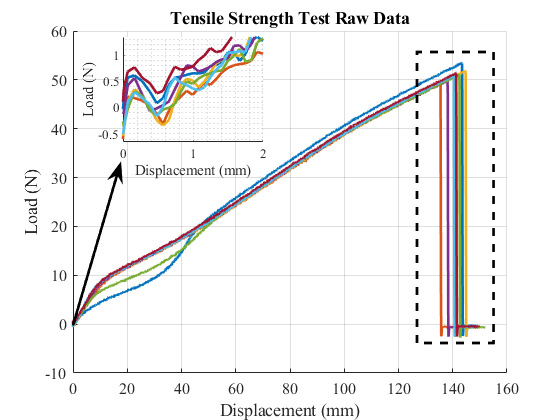
\includegraphics[width=0.93\textwidth]{RawDataToeCompensation.png}
    \caption{Undesired data on the tensile strength results. On the top left, the take-up slack phenomenon at the beginning of the experiment is illustrated. On the right, the different failure points of each specimen from the same material are highlighted.}
    \label{fig:rawData}
\end{figure}

The stress-strain curve from different specimens of the same material is expected to be slightly different from one material to the other, as illustrated in \Cref{fig:rawData}. This variability is caused by many reasons such as the manufacturing process, temperature, and micro fissures inside the material due to handling. For this reason, the engineering ultimate values of stress $\sigma_{ue}$ and strain $\varepsilon_{ue}$ are reported as the median value from all the tests. This variation has an impact on the unification of the data, i.e. creating a single strain-curve by averaging the values from all the tests. In \Cref{fig:unevenData} this impact is illustrated in the form of abrupt changes in the curve around the end section of the curve, caused by the different failing points of each material. The presence of this variation is not critical for the modelling of stage because the material is unlike to be elongated to such high lengths in a real wearable robotic application. However, the decision of discarding this section of the curve in favour of calculating the mean ultimate values of stress $\sigma_u$ and strain $\varepsilon_u$, was made. This section of the curve was also not included when generating the final stress-strain curves of the materials.

%%%%%%%%%%%%%%%%
\begin{figure}[htb!]
    \centering
    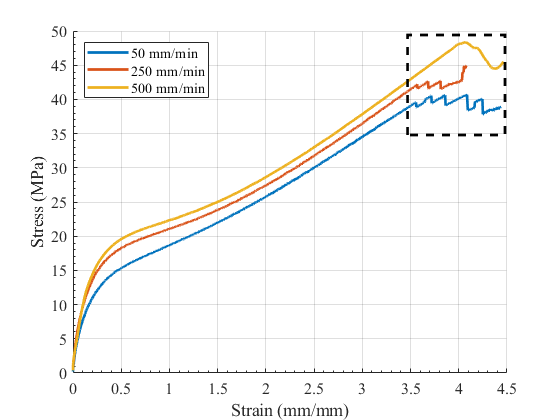
\includegraphics[width=0.7\textwidth]{UnevenUnifiedData.png}
    \caption{Abrupt changes observed at the last portion of the stress-strain curve, caused by the different failure points experimented for each specimen tested.}
    \label{fig:unevenData}
\end{figure}
%%%%%%

The processing algorithm, developed in in Matlab \textregistered{}, was applied to the datasets that exhibit large amount of noise. These datasets were identified by looking at positive and negative peaks, specifically by looking at the mean absolute difference (MAD). Any dataset with a peaks MAD greater than zero was considered noisy and smoothed. The filtering of the noise was done using the \texttt{smoothdata} function with the Savitsky-Sgolay algorithm. This function requires a window parameter to which applied the smoothing algorithm, the larger the window, the greater the smoothing. However, a large window size also introduce a bias or offset to the extreme points of the data. This trade-off is described in \cite{sadeghi2018optimum}. Due to this, the chosen window size was based on the amount of data contained in one second, in this way the window size depends on the different strain rates used because the sampling frequency is constant among all tests. 

The implemented data processing is summarized as follows:
 \begin{enumerate}[noitemsep] %Requires package enumitem
    \item Load raw data from tensile strength tests, i.e. elongation and reaction force (load)
    \item Discard section of the stress-strain curve beyond the failure point
    \item Extract median values of the load and displacement
    \item Discard take-up slack phenomenon
    \item Unify processed data from all specimens into a single dataset by calculating the mean value
    \item Smooth datasets which have a peak-to-peak MAD greater than zero, in the initial portion of the curve
    \item Discard negative offset induced by processing and smoothing
    \item Calculate $\sigma = F/A_o$, and $\varepsilon = l_o/\Delta L$
\end{enumerate}

\subsubsection{Elastic Properties of the Material}

One of the main parameters to extract from the stress-strain curves of the materials is the elastic limit of each material. As previously mentioned in \Cref{sec:mechprop}, this parameter dictates the maximum amount of deformation a material can sustain without losing the ability to fully recover its original shape. Commonly, the proportional limit is used to approximate the location of the elastic limit, and by extension, the elastic region. The proportional limit is the point in the curve where the proportionality between stress and strain becomes nonlinear. It can be safely assumed that the elastic region of the material is located below this point. However, most elastomers do not have a clear elastic region due to their nonlinear stress-strain curve, hence the proportional limit cannot be obtained. Under this circumstance, the elastic region of the material can be approximated using the yield strength of the material. The latter is defined as the first point in the curve where an increment in strain happens without and increment in the stress, in other words when the slope becomes zero or even negative \cite{astmd638}. The yield strength is inside the region of plastic deformations of the material, hence this parameter by itself is not a safe way to approximate the elastic region. 

A better alternative to approximate the elastic region is the offset yield strength. This parameter requires an offset strain value, and the elastic modulus $E$ (slope of the curve) at a specific strain, to be calculated. In the literature, an offset strain of $\varepsilon_{offset}=0.02$, or 2\%, is recommended for plastics and elastomers \cite{instron2019}. This recommendation is mainly to allow comparisons between different laboratories data and does not indicate a goodness of fit when approximating the elastic region or the yield point of a material. In here, we chose a $\varepsilon_{offset}=0.2$ due to the large values of elongation achieved by most of the materials. The main recommendation to calculate $E$ is to choose a strain range inside the initial part of the stress-strain curve in which a linear behaviour can be observed. The elastic modulus is then approximated using a function fitting method such as linear regression. Therefore, the optimal strain range for $E$ was extracted from the obtained stress-strain curves of the materials illustrated in \Cref{fig:EPR-FRSS,fig:NatR-NRSS,fig:PR-SRSS,fig:Nat100RSS}.

In \Cref{fig:EPR-FRSS,fig:NatR-NRSS,fig:PR-SRSS,fig:Nat100RSS}, the stress-strain curve of all the materials studied under different strain rates are presented. The process to obtain the stress-strain curve of the Natural Rubber material was longer than for the other materials, due to the different available thicknesses. These material was extracted from off-the-shelf resistance bands. A total of two different batches were acquired. The measured force response of a band from the same category varied from one batch to the other. The measured thicknesses were not the same among the two batches for a band of the same type. This is directly related to manufacturing practices and is reported in the literature \cite{case2015soft}. For this reason, the individual thickness of each type of rubber band, from each batch was used to convert the raw data to the final stress-strain curve. With this, the impact from the latter differences is decreased and the material behaviour was better captured.
%%%%%%%%%%%%%%%%%%%%%%%%%%%%%%%%%%%%%%%%%%%%%%%%%%%%%%%%%%%%%%%%
\newpage
\begin{figure}[H]
    \centering
        \begin{subfigure}[b]{0.93\textwidth}
        \centering
        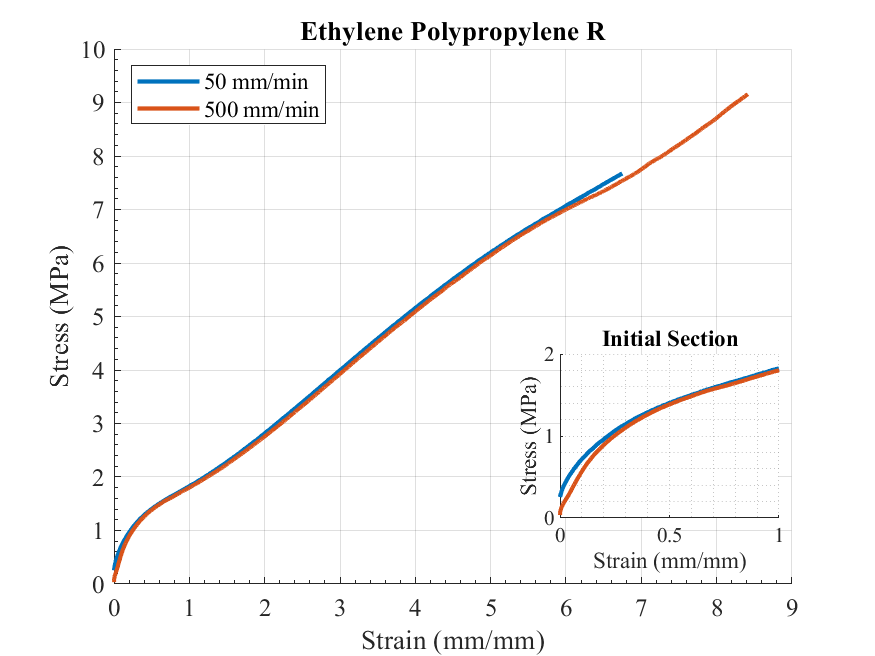
\includegraphics[width=\textwidth]{EPR_StressStrain.png}
        \caption{}
        \label{sfig:EPRSS}
    \end{subfigure}
    \begin{subfigure}[b]{0.93\textwidth}
        \centering
        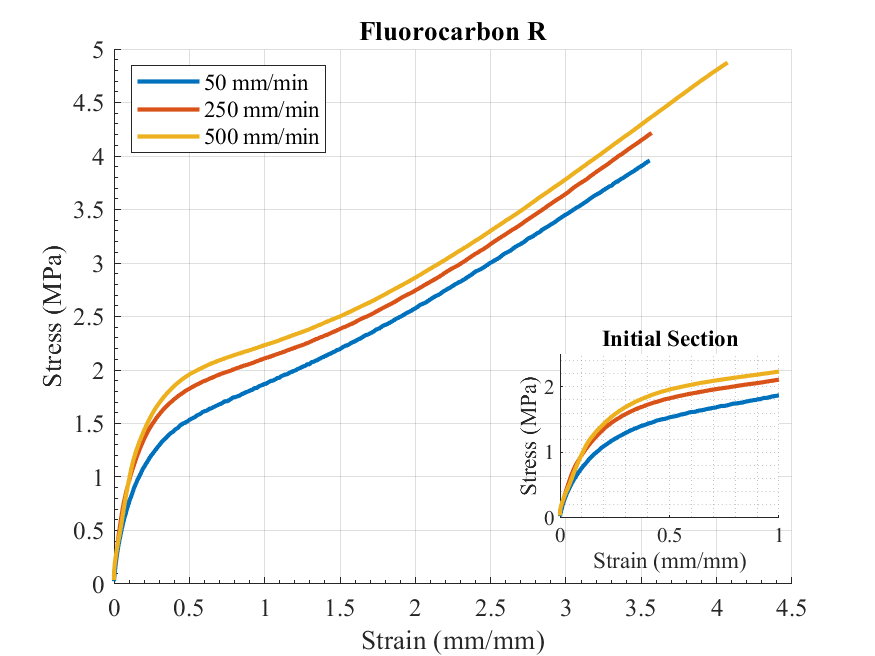
\includegraphics[width=\textwidth]{FR_StressStrain.png}
        \caption{}
        \label{sfig:FRSS}
    \end{subfigure}
    \caption{Stress-strain curves, during different strain rates, for the (a) EPR and (b) FR materials. On the bottom right, the initial section of the curve, where a linear behaviour was observed, is presented.}
    \label{fig:EPR-FRSS}
\end{figure}
\newpage
\begin{figure}[H]
    \centering
    \begin{subfigure}[b]{0.93\textwidth}
    \centering
    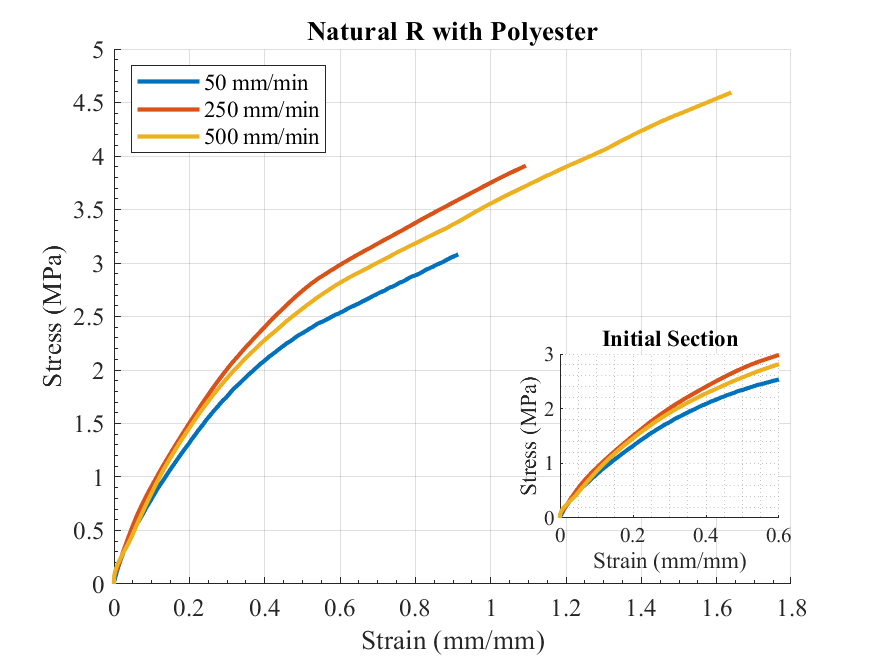
\includegraphics[width=\textwidth]{NatR_StressStrain.png}
    \caption{}
    \label{sfig:NatRSS}
    \end{subfigure}

    \begin{subfigure}[b]{0.93\textwidth}
    \centering
    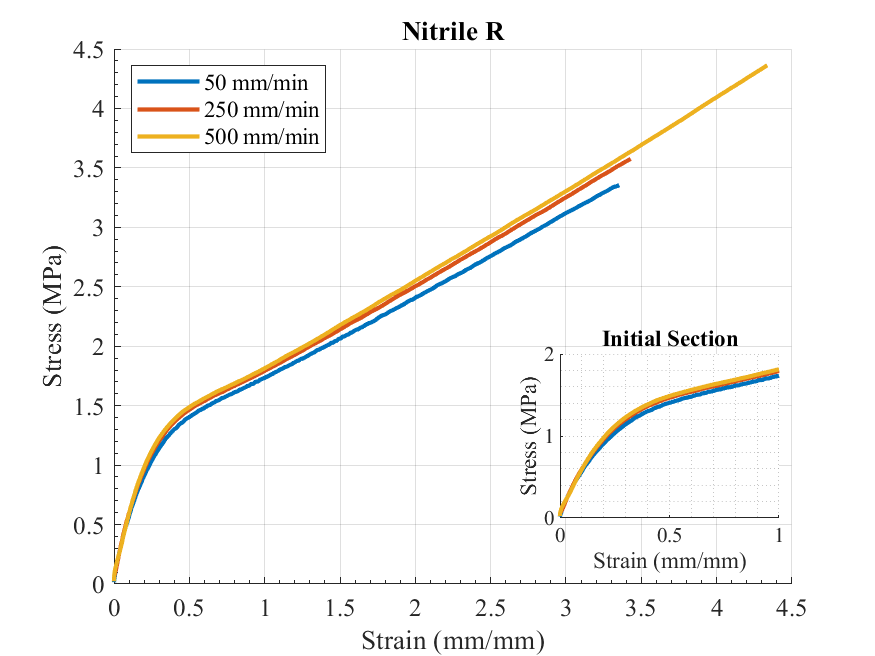
\includegraphics[width=\textwidth]{NR_StressStrain.png}
    \caption{}
    \label{sfig:NRSS}
    \end{subfigure}
    \caption{Stress-strain curves, during different strain rates, for the (a) NatPolR and (b) NR materials. On the bottom right, the initial section of the curve, where a linear behaviour was observed, is presented.}
    \label{fig:NatR-NRSS}
\end{figure}
\newpage
\begin{figure}[H]
    \centering
    \begin{subfigure}[b]{0.93\textwidth}
    \centering
    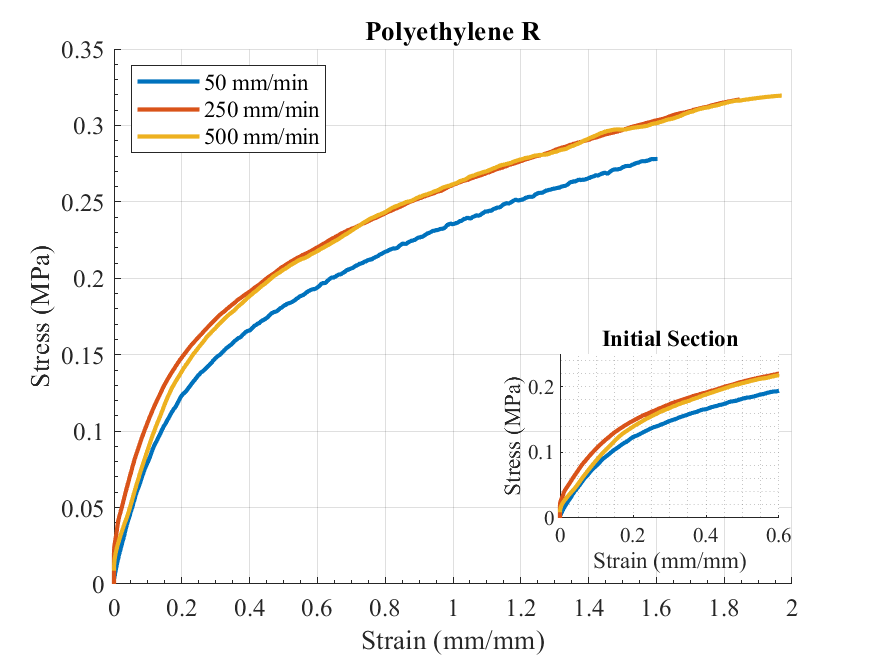
\includegraphics[width=\textwidth]{PR_StressStrain.png}
    \caption{}
    \label{fig:PRSS}
    \end{subfigure}

    \begin{subfigure}[b]{0.93\textwidth}
    \centering
    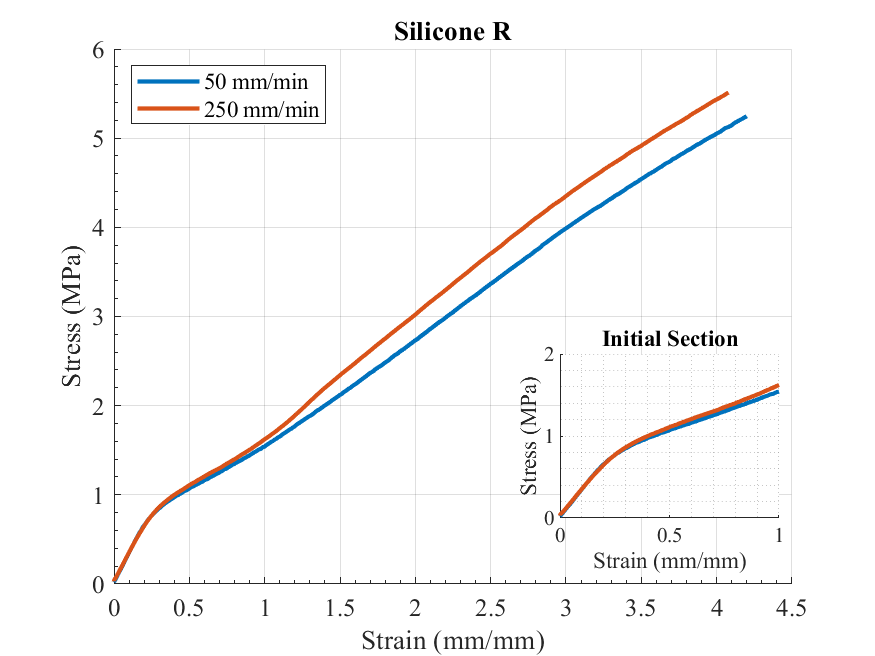
\includegraphics[width=\textwidth]{SR_StressStrain.png}
    \caption{}
    \label{fig:SRSS}
    \end{subfigure}
    \caption{Stress-strain curves, during different strain rates, for the (a) PR and (b) SR materials. On the bottom right, the initial section of the curve, where a linear behaviour was observed, is presented.}
    \label{fig:PR-SRSS}
\end{figure}
\newpage
\begin{figure}[H]
    \vspace*{-2em}
    \centering
    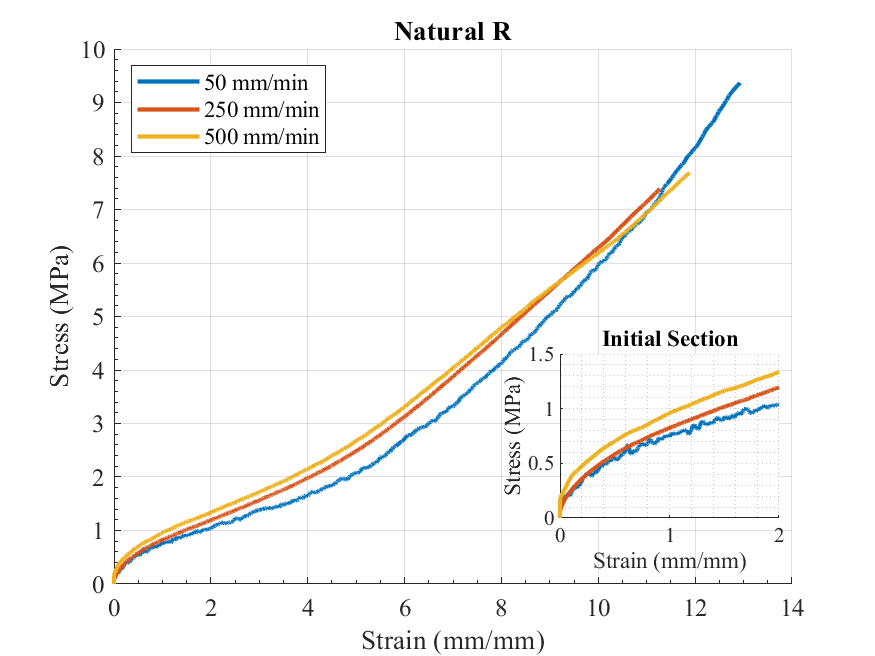
\includegraphics[width=0.93\textwidth]{Nat100R_StressStrain.png}
    \caption{Stress-strain curve, during different strain rates, for the NatR. On the bottom right, the initial section of the curve, where a linear behaviour was observed, is presented.}
    \label{fig:Nat100RSS}
\end{figure}
\vspace*{-1em}
In \Cref{fig:EPR-FRSS,fig:NatR-NRSS,fig:PR-SRSS,fig:Nat100RSS}, the velocity-dependency on the stress response of elastomers can be observed. In general, for larger strain rates, the materials exhibited a larger stress response. Also, the Natural Rubber and Fluorocarbon material showed signs of crystallization, a phenomenon described in \cite{Bauman2008} which happens when the internal molecular chains of the material are completely extended and greatly oppose to further deformation, hence the increase in stiffness just before the failure point. Moreover, most of the materials have two regions in which the proportionality between the stress and strain appears to be constant. This is inline with the expected nonlinear behaviour from elastomers previously described. The slope of these regions, i.e. the stiffness, can be approximated by linear regression. Prior knowledge of the elastic region is required. Therefore, the offset yield strength, $\sigma_y$ and $\varepsilon_y$, is obtained and illustrated in \Cref{fig:FRoff,fig:NatRoff,fig:NRoff,fig:PRoff,fig:Nat100Roff,fig:SR-EPRoff,fig:EPR500off}.

%The correct factor to fit to figures in the same line is 0.49
\newpage
\begin{figure}[H]
    \vspace*{-2em}
    \centering
    \begin{subfigure}[b]{0.65\textwidth}
        \centering
        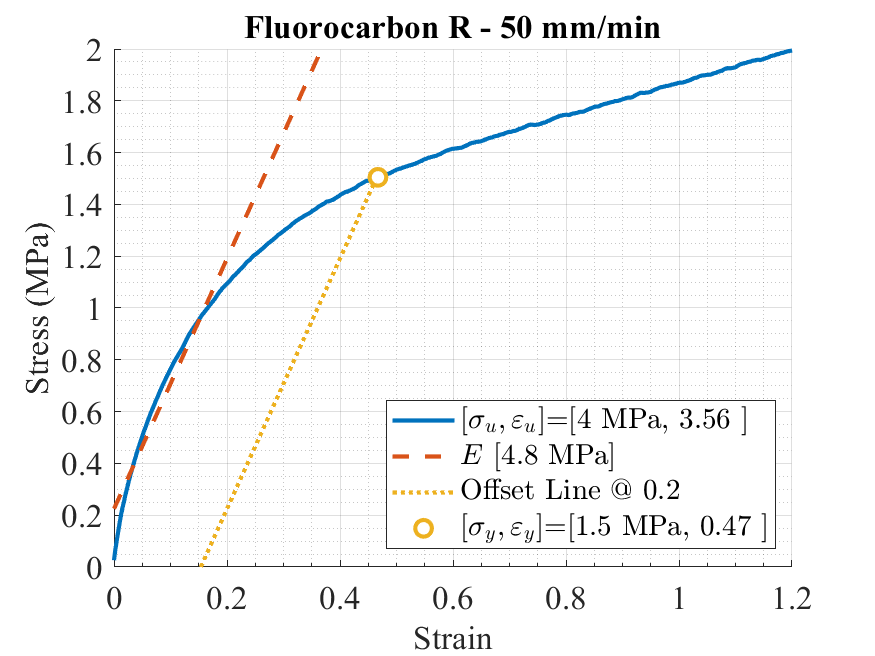
\includegraphics[width=\textwidth]{FR_disR50.png}
        \caption{}
        \label{fig:FR50}
    \end{subfigure}
    \begin{subfigure}[b]{0.65\textwidth}
        \centering
        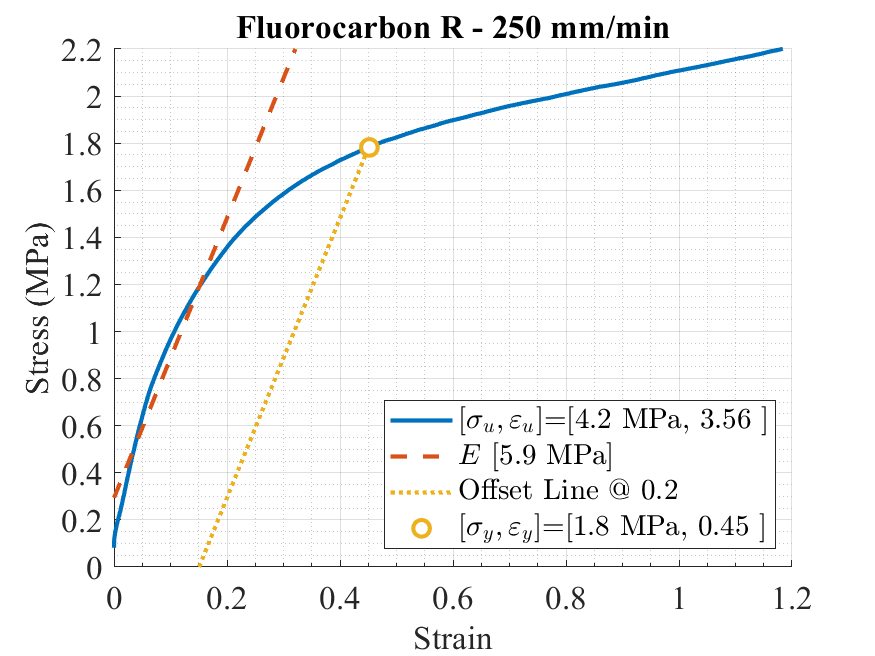
\includegraphics[width=\textwidth]{FR_disR250.png}
        \caption{}
        \label{fig:FR250}
    \end{subfigure}
    \begin{subfigure}[b]{0.65\textwidth}
        \centering
        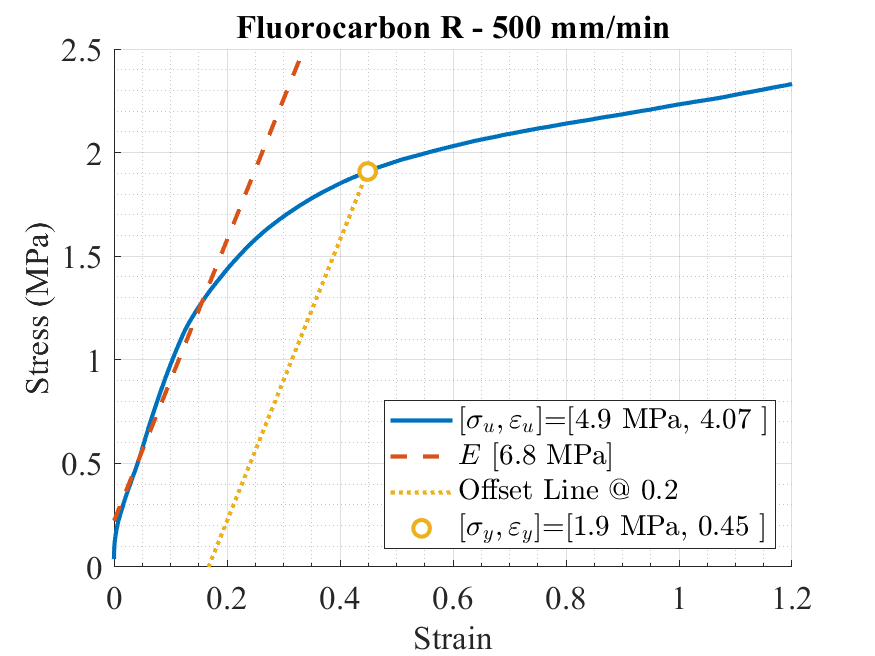
\includegraphics[width=\textwidth]{FR_disR500.png}
        \caption{}
        \label{fig:FR500}
    \end{subfigure}
    \caption{Offset Yield Strength for the FR material}
    \label{fig:FRoff}
\end{figure}
\newpage
\begin{figure}[H]
    \vspace*{-2em}
    \centering
    \begin{subfigure}[b]{0.65\textwidth}
        \centering
        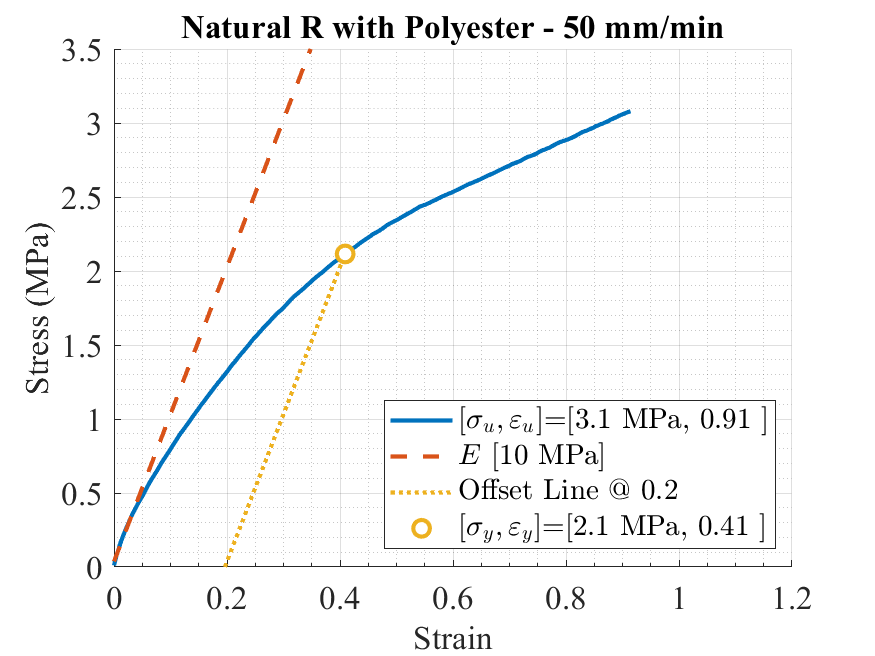
\includegraphics[width=\textwidth]{NatR_disR50.png}
        \caption{}
        \label{fig:NatR50}
    \end{subfigure}
    \begin{subfigure}[b]{0.65\textwidth}
        \centering
        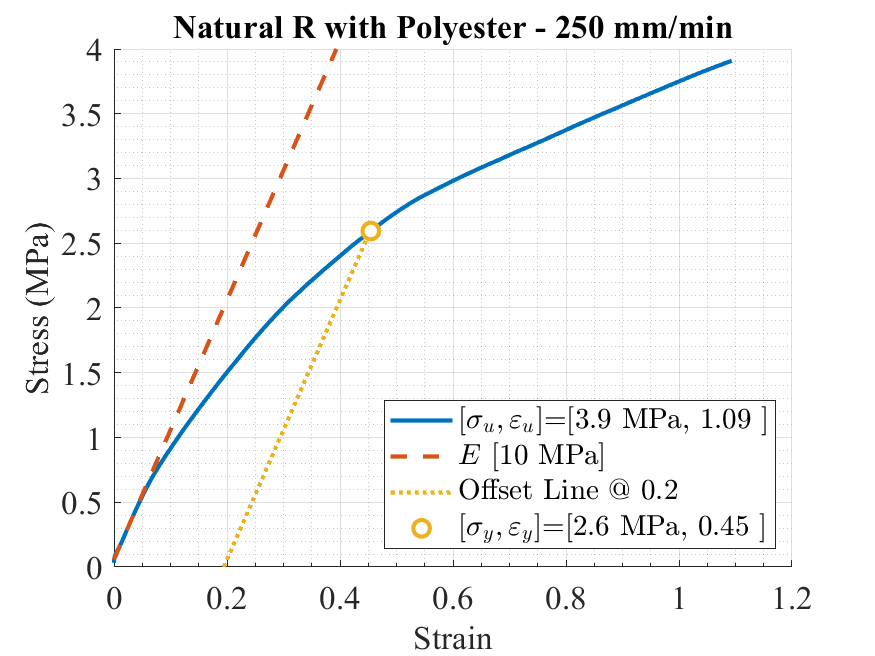
\includegraphics[width=\textwidth]{NatR_disR250.png}
        \caption{}
        \label{fig:NatR250}
    \end{subfigure}
    \begin{subfigure}[b]{0.65\textwidth}
        \centering
        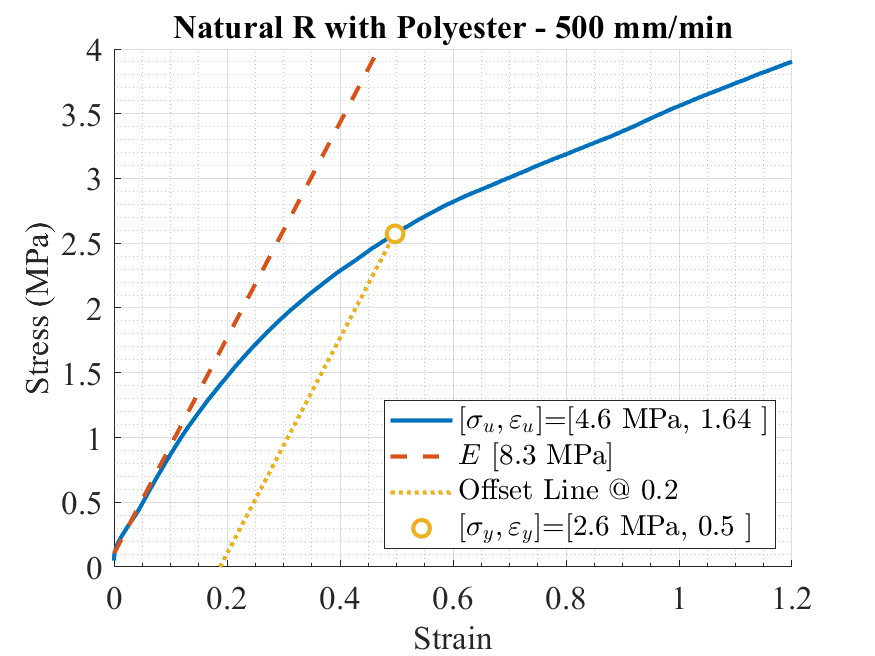
\includegraphics[width=\textwidth]{NatR_disR500.png}
        \caption{}
        \label{fig:NatR500}
    \end{subfigure}
    \caption{Offset Yield Strength for the NatPolR material}
    \label{fig:NatRoff}
\end{figure}
\newpage
\begin{figure}[H]
    \vspace*{-2em}
    \centering
    \begin{subfigure}[b]{0.65\textwidth}
        \centering
        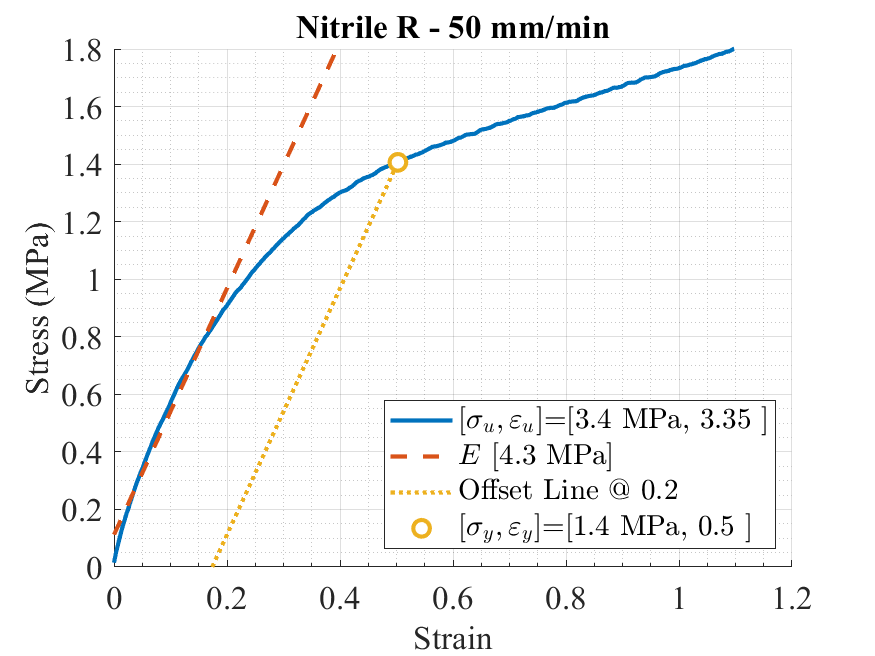
\includegraphics[width=\textwidth]{NR_disR50.png}
        \caption{}
        \label{fig:NR50}
    \end{subfigure}
    \begin{subfigure}[b]{0.65\textwidth}
        \centering
        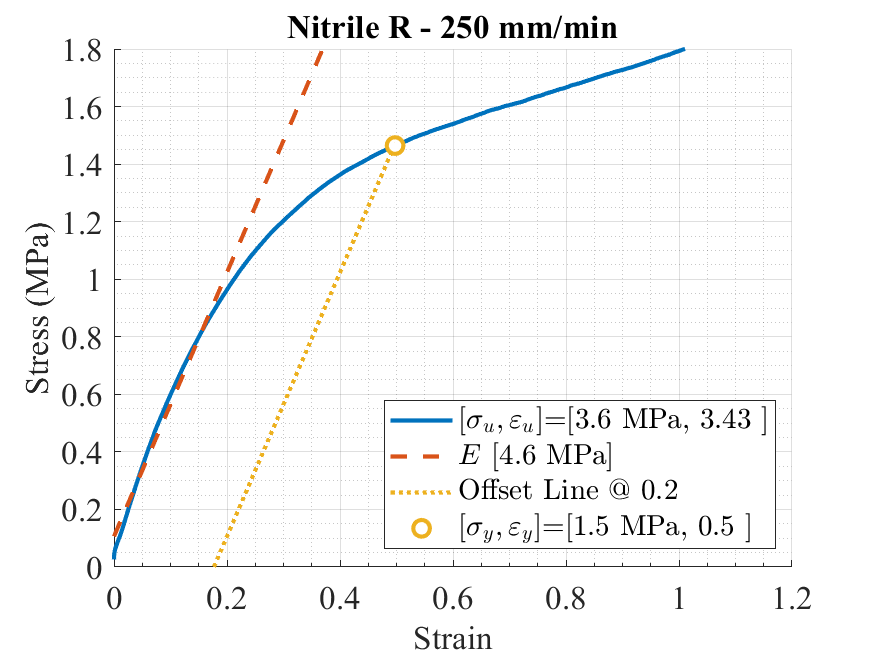
\includegraphics[width=\textwidth]{NR_disR250.png}
        \caption{}
        \label{fig:NR250}
    \end{subfigure}
    \begin{subfigure}[b]{0.65\textwidth}
        \centering
        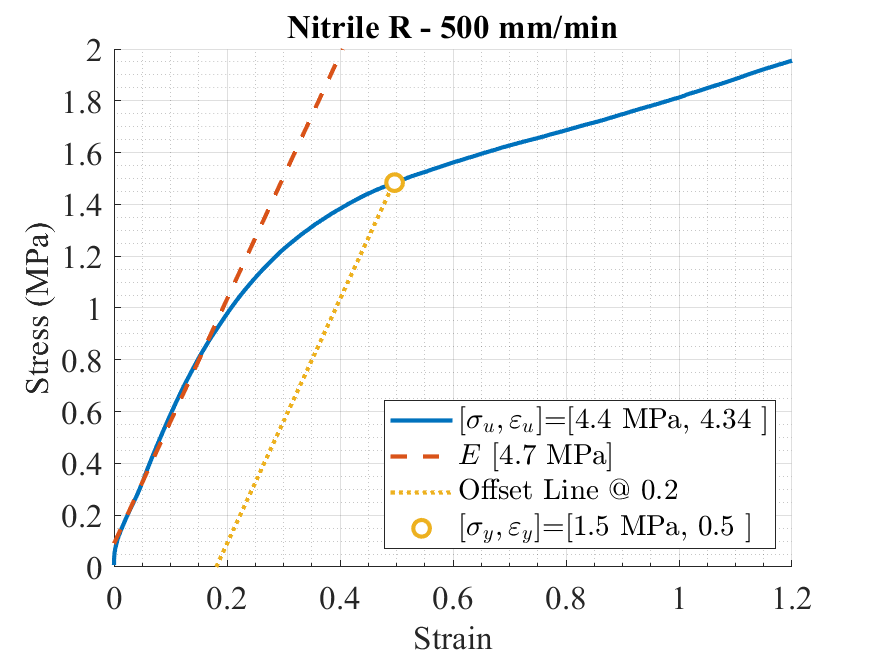
\includegraphics[width=\textwidth]{NR_disR500.png}
        \caption{}
        \label{fig:NR500}
    \end{subfigure}
    \caption{Offset Yield Strength for the NR material}
    \label{fig:NRoff}
\end{figure}
\newpage
\begin{figure}[H]
    \vspace*{-2em}
    \centering
    \begin{subfigure}[b]{0.65\textwidth}
        \centering
        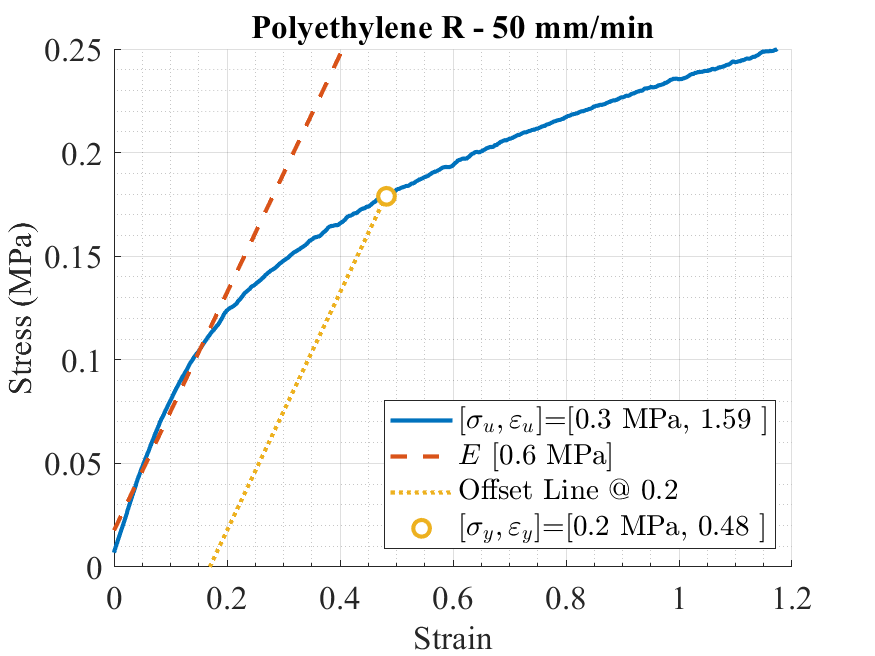
\includegraphics[width=\textwidth]{PR_disR50.png}
        \caption{}
        \label{fig:PR50}
    \end{subfigure}
    \begin{subfigure}[b]{0.65\textwidth}
        \centering
        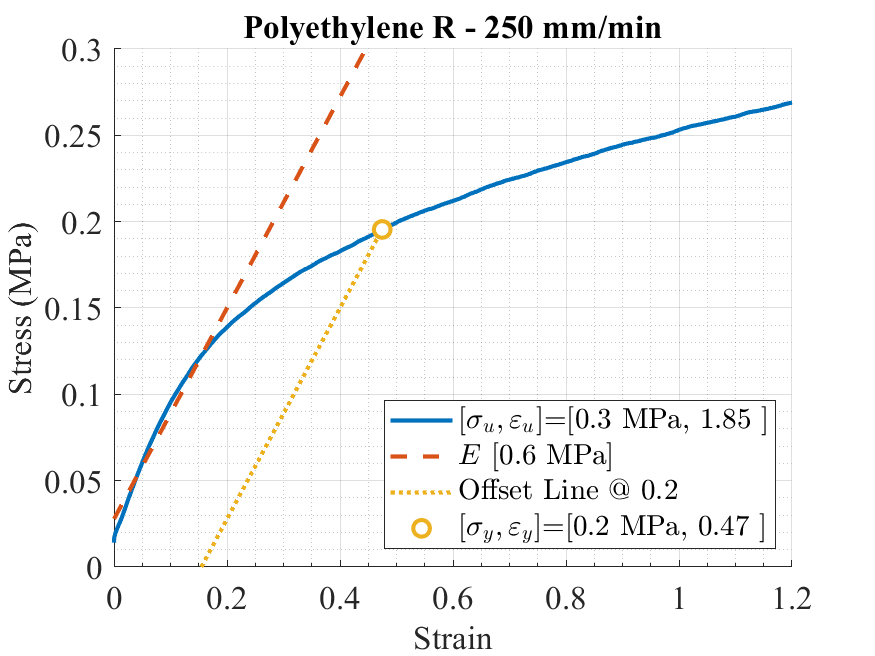
\includegraphics[width=\textwidth]{PR_disR250.png}
        \caption{}
        \label{fig:PR250}
    \end{subfigure}
    \begin{subfigure}[b]{0.65\textwidth}
        \centering
        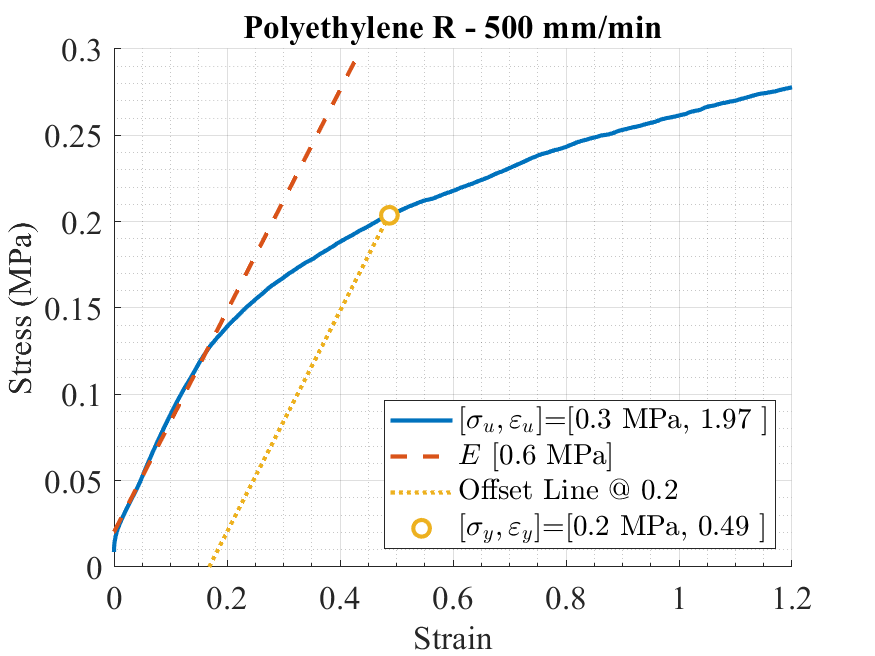
\includegraphics[width=\textwidth]{PR_disR500.png}
        \caption{}
        \label{fig:PR500}
    \end{subfigure}
    \caption{Offset Yield Strength for the PR material}
    \label{fig:PRoff}
\end{figure}
\newpage
\begin{figure}[H]
    \vspace*{-2em}
    \centering
    \begin{subfigure}[b]{0.65\textwidth}
        \centering
        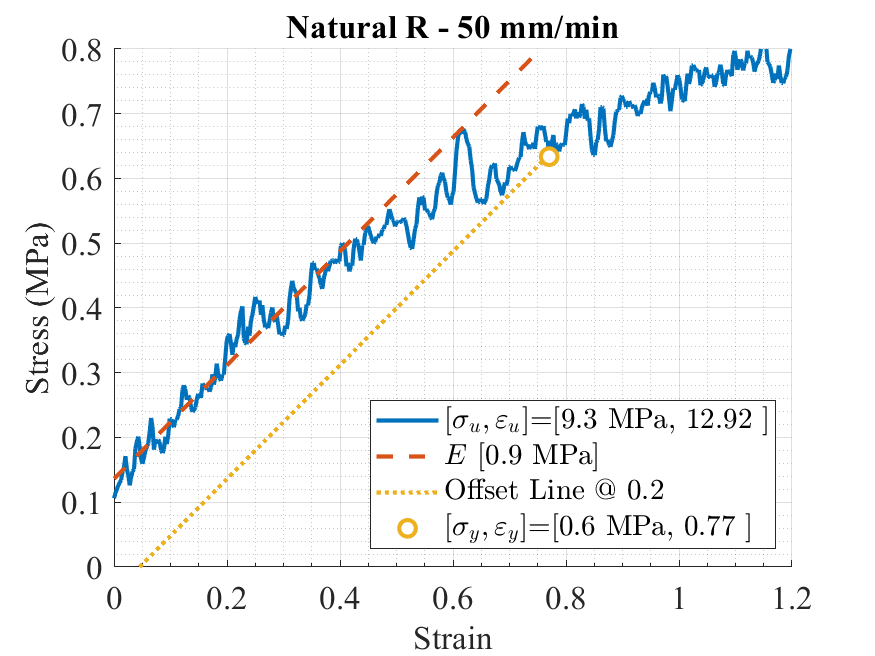
\includegraphics[width=\textwidth]{Nat100R_disR50.png}
        \caption{}
        \label{fig:Nat100R50}
    \end{subfigure}
    \begin{subfigure}[b]{0.65\textwidth}
        \centering
        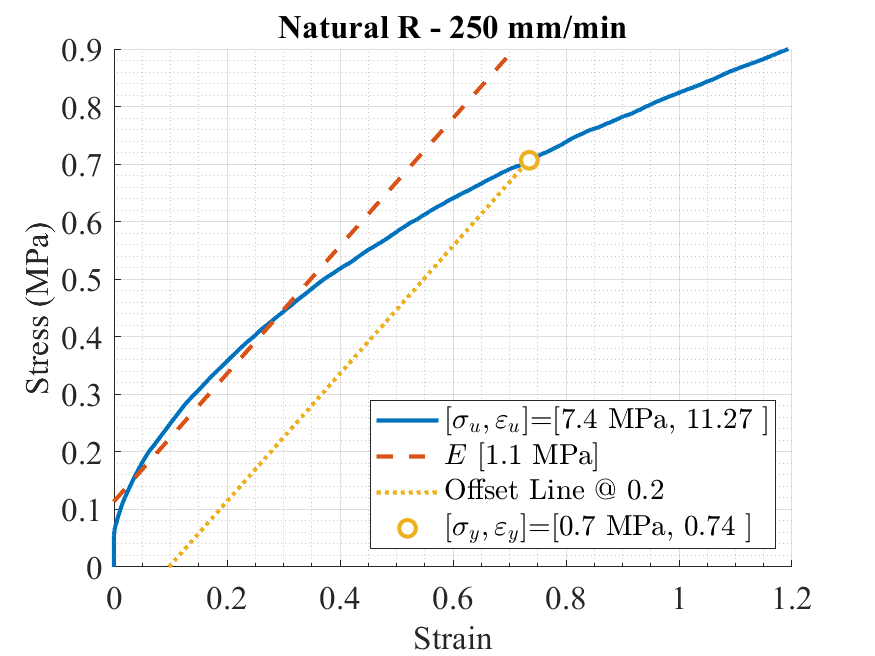
\includegraphics[width=\textwidth]{Nat100R_disR250.png}
        \caption{}
        \label{fig:Nat100R250}
    \end{subfigure}
    \begin{subfigure}[b]{0.65\textwidth}
        \centering
        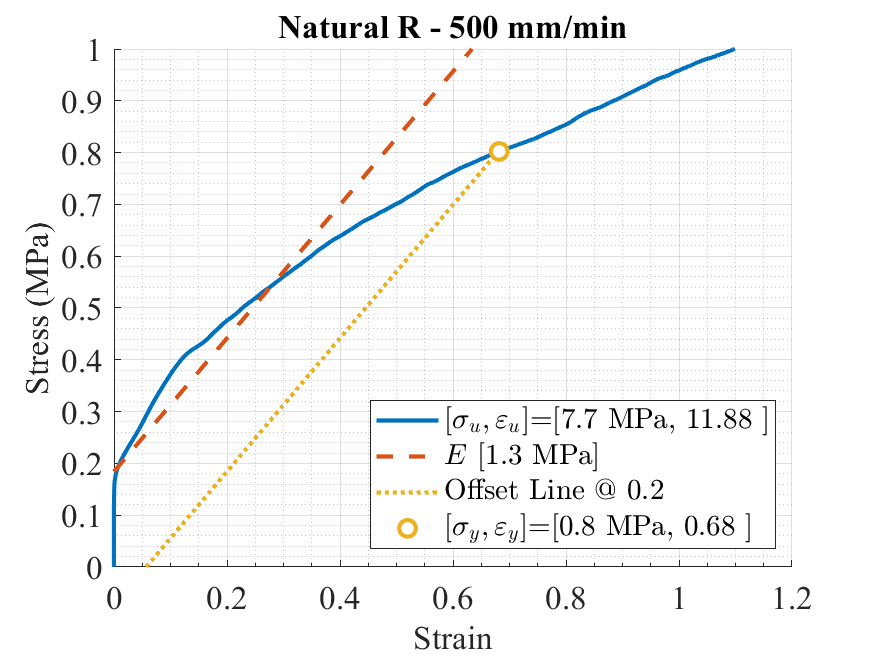
\includegraphics[width=\textwidth]{Nat100R_disR500.png}
        \caption{}
        \label{fig:Nat100R500}
    \end{subfigure}
    \caption{Offset Yield Strength for the NatR material}
    \label{fig:Nat100Roff}
\end{figure}
\newpage
\begin{figure}[H]
    \vspace*{-2em}
    \centering
    \begin{subfigure}[b]{0.65\textwidth}
        \centering
        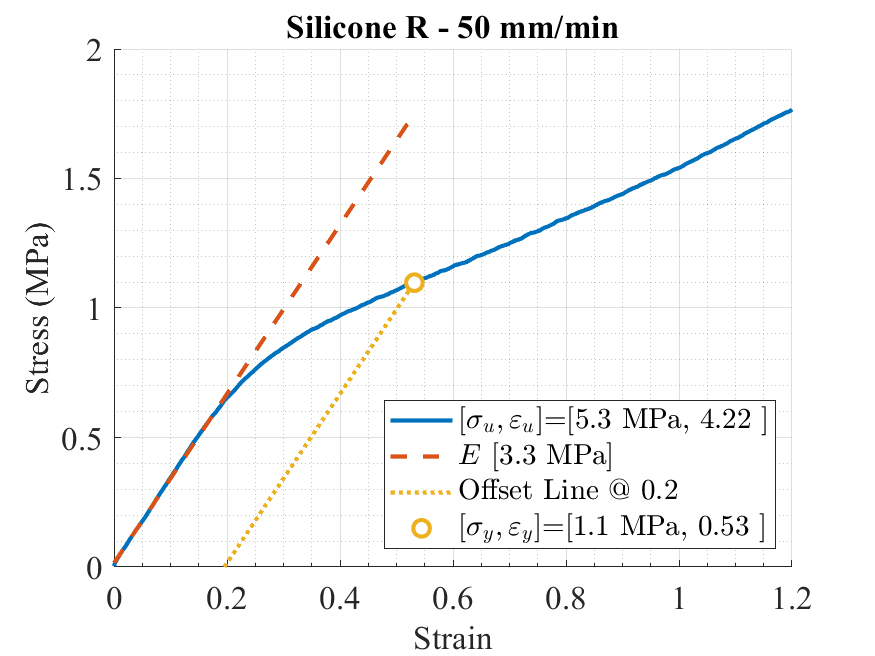
\includegraphics[width=\textwidth]{SR_disR50.png}
        \caption{}
        \label{fig:SR50}
    \end{subfigure}
    \begin{subfigure}[b]{0.65\textwidth}
        \centering
        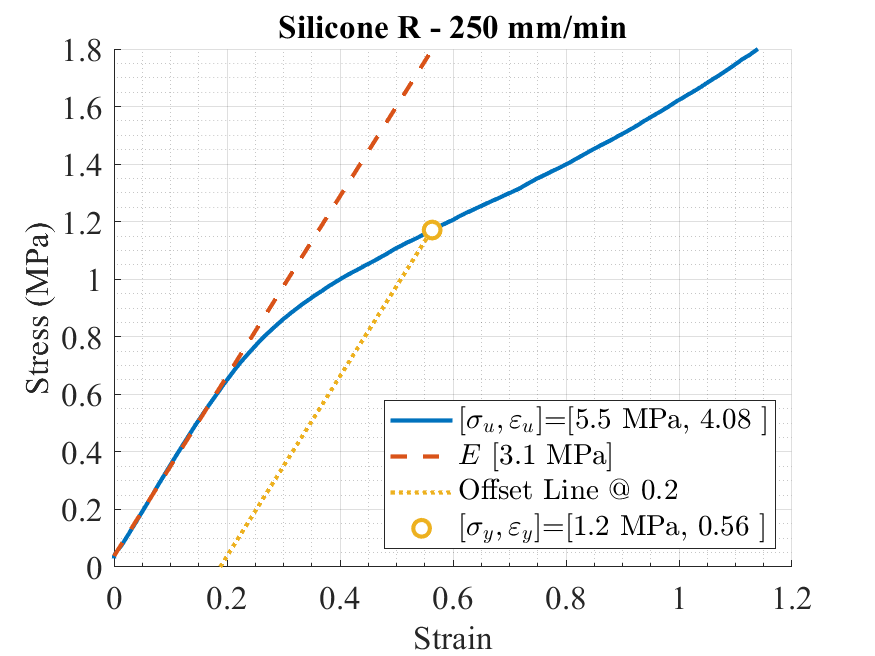
\includegraphics[width=\textwidth]{SR_disR250.png}
        \caption{}
        \label{fig:SR250}
    \end{subfigure}
    \begin{subfigure}[b]{0.65\textwidth}
        \centering
        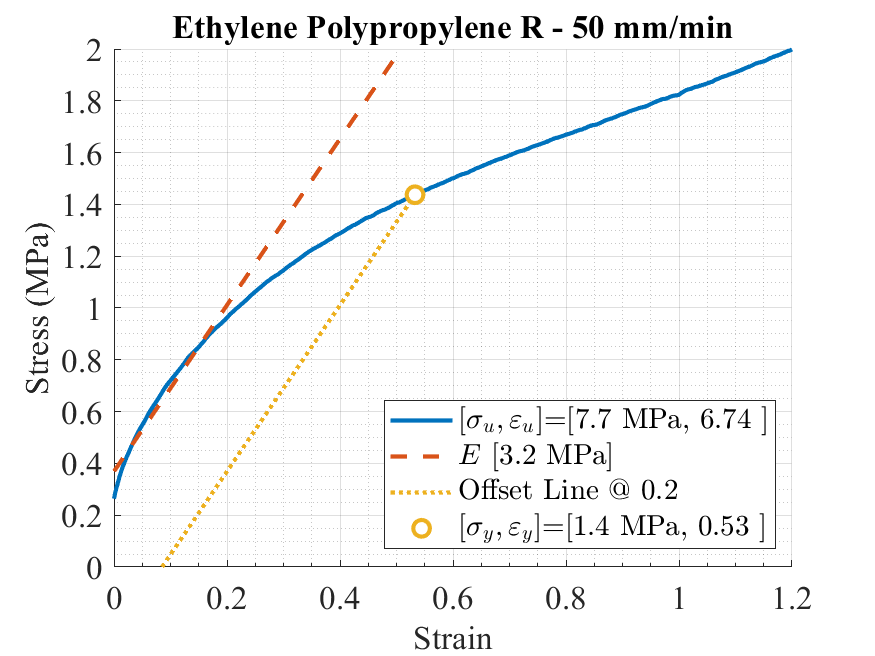
\includegraphics[width=\textwidth]{EPR_disR50.png}
        \caption{}
        \label{fig:EPR50}
    \end{subfigure}
    \caption{Offset Yield Strength for the SR and EPR (50mm/min) material.}
    \label{fig:SR-EPRoff}
\end{figure}
\begin{figure}[H]
    \vspace*{-2em}
    \centering
    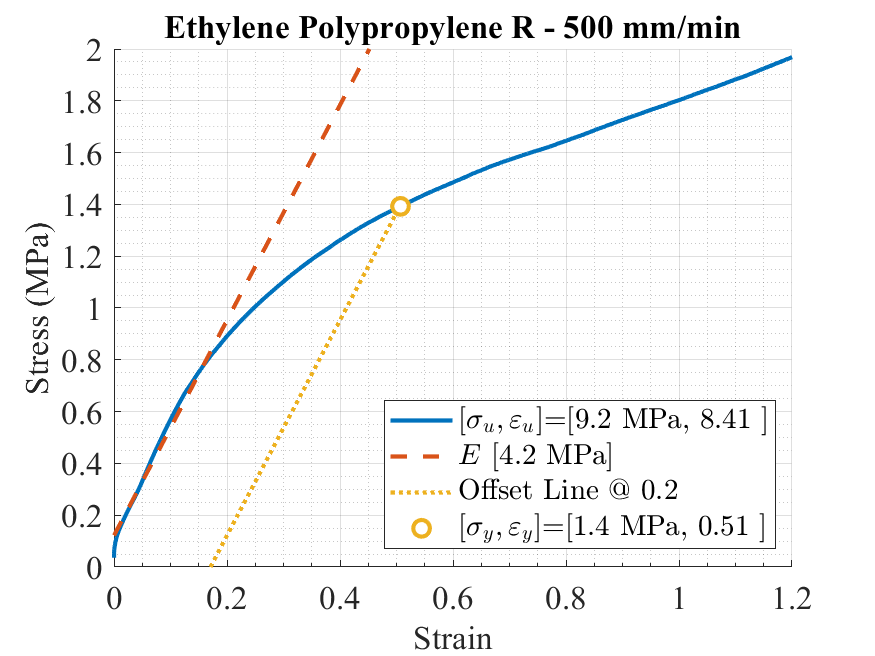
\includegraphics[width=0.65\textwidth]{EPR_disR500.png}
    \caption{Offset Yield Strength for the EPR (500mm/min) material}
    \label{fig:EPR500off}
\end{figure}

In \Cref{fig:FRoff,fig:NatRoff,fig:NRoff,fig:PRoff,fig:Nat100Roff,fig:SR-EPRoff,fig:EPR500off}, the elastic region is approximated by using the offset yield strength parameter. Also, the values for the ultimate strength, yield strength, and the elastic modulus at the elastic region, are provided. Any value below the offset yield strain can be assumed to be inside the elastic region of the material, hence the material will recover its original shape after undergoing any deformation inside this range of values. Having delimited the elastic region and its elastic modulus (now $E_{small}$), the slope of the second linear portion of the curve, i.e. the elastic modulus $E_{large}$, can be approximated. Finally, the elastic properties of the material are compiled in \Cref{tbl:elasticProp}.

In \Cref{tbl:elasticProp}, the $\sigma_{ue}$ and $\varepsilon_{ue}$ are reported as the median value from the all the specimens of a specific test type. The yield values $\sigma_{y}$ and $\varepsilon_{y}$ were obtained using the offset yield strength method. The parameters $E_{small}$ and $E_{large}$ are the elastic modulus at the initial section, and middle section of the stress-strain curve. Also, $E_{small}$ is the most useful parameter for assessing the performance of a material in a real robotic application, because it describes the stiffness of a material inside the elastic region, i.e. safe working conditions. In this regards the PR material had the smallest value, whereas the NatR had the highest.

% The detailed process to calculate the offset yield strength is as follows. The first step is to apply a linear regression to the first part of the stress-strain curve. In this work, the range from 0 to 20\% strain is chosen. The slope of the fitted line represents the elastic modulus at the specified strain (20. The second step is to create a new line, starting from the specified 2\% offset strain, using the previously found elastic modulus as its slope. Finally, this line is projected up to the point in which it intersects the stress-strain curve. The stress and strain at this point represent the offset yield stress and the offset yield strain, respectively. Therefore, it is assume that beyond this point the material start undergoing plastic deformations. Similarly, it is assumed that the material is able to recover its original shape for all deformations found bellow the offset yield strain. 

\begin{table*}[htb!]
\centering
\caption{Elastic properties of the selection of soft materials.}
\label{tbl:elasticProp}
\begin{tabular}{lccccccccc} \toprule
Materials                  & Speed & $\sigma_{ue}$ & $\varepsilon_{ue}$ & $\sigma_{u}$ & $\varepsilon_{u}$ & $\sigma_{y}$ & $\varepsilon_{y}$ & $E_{small}$ & $E_{large}$ \\
                           & mm/min   & MPa &  & MPa &  & MPa &  & MPa & MPa \\
\hline
\multirow{2}{*}{EPR}      & 50    & 8.48       & 7.56       & 7.67    & 6.74    & 1.44    & 0.54    & 3.23     & 0.99      \\
                           & 500   & 9.59       & 8.84       & 9.16    & 8.41    & 1.39    & 0.51    & 4.16     & 1.1       \\
\hline
\multirow{3}{*}{FR}      & 50    & 4.36       & 3.97       & 3.96    & 3.56    & 1.5     & 0.47    & 4.83     & 0.65      \\
                           & 250   & 4.41       & 3.93       & 4.22    & 3.57    & 1.78    & 0.45    & 5.95     & 0.58      \\
                           & 500   & 5.35       & 4.29       & 4.87    & 4.07    & 1.91    & 0.45    & 6.78     & 0.61      \\
\hline
\multirow{3}{*}{NatPolR}    & 50    & 3.57       & 1.19       & 3.08    & 0.91    & 2.12    & 0.41    & 9.97     & 2.05      \\
                           & 250   & 4.06       & 1.19       & 3.91    & 1.09    & 2.51    & 0.43    & 10.74    & 2.28      \\
                           & 500   & 4.59       & 1.64       & 4.59    & 1.64    & 2.52    & 0.48    & 8.77     & 1.9       \\
\hline
\multirow{3}{*}{NR}      & 50    & 3.55       & 3.57       & 3.36    & 3.36    & 1.41    & 0.5     & 4.29     & 0.64      \\
                           & 250   & 3.65       & 3.62       & 3.58    & 3.43    & 1.47    & 0.5     & 4.63     & 0.69      \\
                           & 500   & 4.62       & 4.61       & 4.37    & 4.34    & 1.48    & 0.5     & 4.72     & 0.72      \\
\hline
\multirow{3}{*}{PR}      & 50    & 0.3        & 1.87       & 0.28    & 1.59    & 0.18    & 0.48    & 0.58     & 0.11      \\
                           & 250   & 0.33       & 1.97       & 0.31    & 1.83    & 0.19    & 0.45    & 0.66     & 0.1       \\
                           & 500   & 0.32       & 1.97       & 0.32    & 1.97    & 0.2     & 0.49    & 0.64     & 0.1       \\
\hline
\multirow{2}{*}{SR}      & 50    & 6.03       & 5.77       & 5.26    & 4.22    & 1.1     & 0.53    & 3.26     & 1.08      \\
                           & 250   & 5.68       & 4.27       & 5.52    & 4.08    & 1.15    & 0.54    & 3.26     & 1.35      \\
\hline
\multirow{3}{*}{NatR} & 50    & 9.43       & 13.02      & 9.37    & 12.93   & 0.61    & 0.69    & 1.01     & 0.33      \\
                           & 250   & 15.88      & 12.11      & 7.38    & 11.27   & 0.69    & 0.74    & 1.11     & 0.41      \\
                           & 500   & 11.93      & 12.26      & 6.61    & 11.22   & 0.73    & 0.71    & 1.19     & 0.43     \\
\bottomrule
\end{tabular}
\end{table*}


\subsection{Stress Relaxation Test}

The stress relaxation test allows the extraction of the viscoelastic properties of the materials, i.e. the time-dependent properties. In this test, a predefined and constant elongation, also called initial strain $\varepsilon_o$ is applied to the material specimen. The material is hold in place for the whole duration of the test and the stress response is recorded. The material will relax over time, i.e. the stress response will decrease. Similarly as for the tensile strength test, different combinations of test duration and initial strain values were chosen to test the materials. Also, a varying number of specimens were included in each test. Some of these combinations were based on similar characterization processes available in the literature \cite{case2015soft,delin1995volume}. As a recommendation, the value for the applied $\varepsilon_o$ must be fall beyond the elastic region of the material to avoid plastic deformation, i.e. irreparable damage. However, for highly elastic materials, such as elastomers, large values of $\varepsilon_o$ are used in the literature. Also, the material must be elongated from zero strain to the value of $\varepsilon_o$ as fast as possible. Therefore, the strain rate chosen for this test was  500 mm/min. The parameters for the performed tests are compiled in \Cref{tbl:stressRelParameters}.

\begin{table*}[htb!]
\centering
\caption{Parameters and number of collected datasets for the stress relaxation tests.}
\label{tbl:stressRelParameters}
\begin{tabular}{llccccccc} \toprule
Test & Parameters & EPR & FR & NatPolR & NR & PR & SR & NatR \\
\hline
\multirow{3}{*}{1}  & $\varepsilon_o$ (mm)      & 5 & 5 & 7 & 6 & 3 & 6 & 40 \\
                    & Duration (minutes)    & 15 & 15 & 15 & 15 & 15 & 15 & 15 \\
                    & Datasets              & 5 & 5 & 5 & 5 & 5 & 5 & 2 \\
\hline 
\multirow{3}{*}{2}  & $\varepsilon_o$ (mm)      & 20 & 10 & 6 & 5 & 4 & 15 & - \\
                    & Duration (minutes)    & 180 & 180 & 180 & 180 & 180 & 180 & 180 \\
                    & Datasets              & 1 & 1 & 1 & 1 & 1 & 1 & - \\
\bottomrule
\end{tabular}
\end{table*}

\subsubsection{Data Processing}

Similarly to the tensile strength tests, the collected data was processed prior to the extraction of the relevant parameters. The data of interest is the one found after the machine has reached the predefined $\varepsilon_o$ value. In here, several smoothing algorithms such as, moving average, Gaussian-weighted moving average, and the Savitzky-Golay algorithm, were analyzed. During testing of these algorithm, a direct relationship between the decrease in the value of the initial stress $\sigma_o$, and the selected window size, was observed. The selected window size was based on the sampling frequency and the duration of the test. The Savitzky-Golay algorithm performed better than the other two algorithms.

\subsubsection{Stress Relaxation Properties}

The stress relaxation test is useful for approximating the time relaxation constants of the materials. Commonly, viscoelastic materials have more than one relaxation constant. This is caused by the many number of internal molecular chains which relax at different rates. The stress relaxation curve of viscoelastic materials exhibit a decaying exponential stress relaxation curve. This known mathematical function, in combination with the LVMs, can be used to approximate the time relaxation constants of the material. The LVMs have the flexibility to get as complex as required by adding extra elements to the model. This latter means that the number of relaxation constants that can be extracted from the stress relaxation curve is directly proportional to the number of exponential functions contained in the LVM. This is described in detail in \Cref{sec:ModellingLVM}.

The stress at the starting and ending point of the test,  $\sigma_o$ and $\sigma_{end}$ respectively, are the minimum required parameters to approximate one relaxation constant of the material using a LVM. The achieved stress relaxation is defined by, $S.R. = 100(\sigma_o - \sigma_{end}/\sigma_o)$. Hence, the extracted properties of the materials are compiled in \Cref{tbl:stressRelProperties}. Also, the obtained stress relaxation curves of all the materials are illustrated in \Cref{fig:AllSRel,fig:PRSRel}.

\begin{table*}[htb!]
\centering
\caption{Stress relaxation properties for the selection of soft materials.}
\label{tbl:stressRelProperties}
\begin{tabular}{llccccccc} \toprule
Test & Properties & EPR & FR & NatPolR & NR & PR & SR & NatR \\
\hline
\multirow{3}{*}{1}  & $\sigma_o$ (MPa)   & 0.61      & 0.84      & 1.22      & 0.77      & 0.06      & 0.61      & 2.15 \\
                & $\sigma_{end}$ (MPa)    & 0.42      & 0.27      & 0.80      & 0.55      & 0.02      & 0.43      & 1.82 \\
                & $S.R. (\%)$    &  32     & 67      & 35      & 29      & 63      & 31      & 15 \\
                     
\hline 
\multirow{3}{*}{2}  & $\sigma_o$ (MPa)     & 1.28      & 1.13      & 1.18      & 0.72      & 0.07      & 1.11  &         \\
                & $\sigma_{end}$ (MPa)     & 0.89      & 0.41      & 0.76      & 0.55      & 0.03      & 0.80  &          \\
                & $S.R. (\%)$     & 31      & 63      & 36      & 24      & 51      & 28  &          \\
\bottomrule
\end{tabular}
\end{table*}


\begin{figure}[H]
    \centering
        \begin{subfigure}[b]{0.93\textwidth}
        \centering
        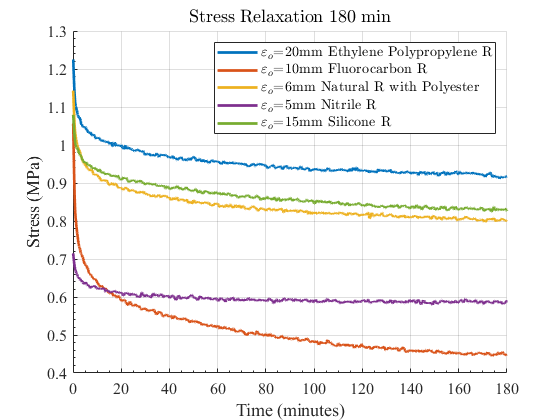
\includegraphics[width=\textwidth]{All180SRel.png}
        \caption{Caption}
        \label{sfig:ALL180SRel}
    \end{subfigure}
    \begin{subfigure}[b]{0.93\textwidth}
        \centering
        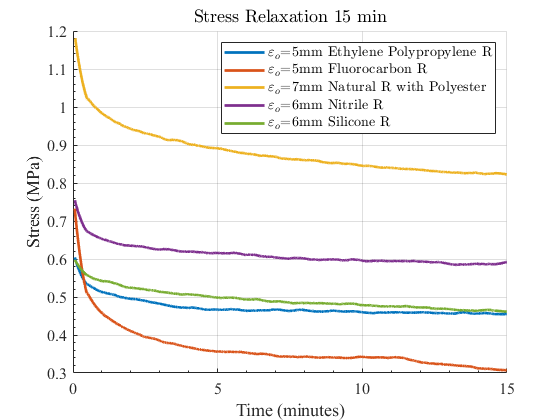
\includegraphics[width=\textwidth]{All15SRel.png}
        \caption{Caption}
        \label{sfig:centering}
    \end{subfigure}
    \caption{Caption}
    \label{fig:AllSRel}
\end{figure}

\newpage
\begin{figure}[H]
    \centering
        \begin{subfigure}[b]{0.93\textwidth}
        \centering
        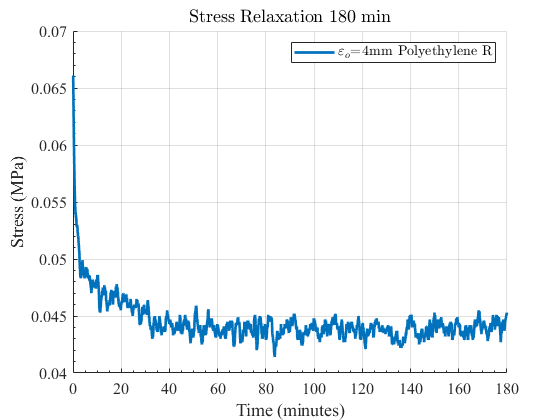
\includegraphics[width=\textwidth]{PR180SRel.png}
        \caption{Caption}
        \label{sfig:PR180SRel}
    \end{subfigure}
    \begin{subfigure}[b]{0.93\textwidth}
        \centering
        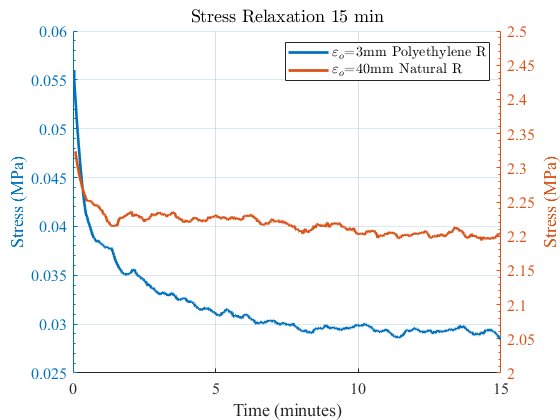
\includegraphics[width=\textwidth]{PR15SRel.png}
        \caption{Caption}
        \label{sfig:PR15SRel}
    \end{subfigure}
    \caption{Caption}
    \label{fig:PRSRel}
\end{figure}

The values of $\sigma_o$ and $\sigma_{end}$ reported in \Cref{tbl:stressRelProperties}, were obtained by finding the median of the tested specimens per type of test. This is done prior to the smoothing of the data. The reported values for the achieved $S.R.$ are very similar in both tests, regarding of the duration of the test and the chosen $\varepsilon_o$. This suggest that most of the S.R. happens very early into the test. This, at the same time, could indicate that only one relaxation time constant is required to model the stress relaxation of these materials. Finally, the obtained curves are illustrated in \Cref{fig:AllSRel,fig:PRSRel}, where a quick drop in the stress response is observed at the initial portion of the curve.

%In this paragraph I could mention that depending on the linearity of the stress relaxation curve plotted in logarithmic scale, one can assume how many relaxation times are present. This part could be more suitable on the modelling chapter.

%More information on the stress relaxation modulus can be found in the Book Engineering Viscoelasticity. Although, the relevance of bringing this information in here is not clear.

\section{Summary}

In this chapter, the characterization process of the viscoelastic mechanical properties of a selection of seven different TPEs was presented. For this, the mechanical tests of tensile strength and stress relaxation was performed. In the tensile strength test, the materials were elongated until failure using up to three different strain, or elongation, rates. The latter will allow the modeling of the velocity-dependent stress response of the materials. The processing algorithm used to condition the collected data was also described in detail. The smoothing algorithm chosen for both mechanical tests was the Savitsky-Sgolay algorithm. In the case for the Natural Rubber material, where two batches were acquired, the thickness from one batch to the other varied significantly. Nevertheless, the mechanical behaviour of the material was captured accurately in the stress-strain curves. This suggest a linear proportionality between the thickness of the material and the increment on the response fore of the material. The elastic region of the materials was difficult to be identified directly due their nonlinear stress-strain curve. Therefore, the elastic region was approximated using the offset yield strength parameter. This region is very important to delimit the working conditions of the soft materials in a real robotic application. Finally, the ultimate values of strain and stress, the elastic region location, the elastic modulus in two distinctive regions of the curve, and the offset yield strength parameters, were reported. The $E_{small}$ is the most useful parameter for assessing the performance of a material in a real robotic application, because it describes the stiffness of a material inside the elastic region, i.e. safe working conditions, in contrast to the ultimate strength values. In this regards the PR material had the smallest value, whereas the NatR had the highest.

The performed stress relaxation tests can be divided in two sets. One with a low deformation, and low duration. The other, with large deformation, large duration. Regarding of this, the achieved stress relaxation of the materials was very similar for both cases. Knowing the resemblance of the stress relaxation curve with an exponential decaying function, the latter finding could suggest that only one relaxation time constant is responsible for the majority of the $S.R.$ achieved.  This hypothesis will be explored in the modeling stage. 

%Finish this chapter by: Checking Captions. Additionally, make each chapter start on an even page. Plots need to be redone